\documentclass{scrartcl}
\usepackage[utf8]{inputenc}
\usepackage[T1]{fontenc}
\usepackage[a4paper]{geometry}
\usepackage{graphicx}
\usepackage{hyperref}
\usepackage{float}
\usepackage{mathtools}
\usepackage{textcomp}
\usepackage{gensymb}
\usepackage[ngerman]{babel}
\usepackage{epstopdf}
\usepackage{titlesec}
\renewcommand{\arraystretch}{1.3}
\setcounter{secnumdepth}{5}
\setcounter{tocdepth}{5}
\makeatletter
\renewcommand\paragraph{\@startsection{paragraph}{4}{\z@}%
  {-3.25ex\@plus -1ex \@minus -.2ex}%
  {1.5ex \@plus .2ex}%
  {\normalfont\normalsize\bfseries}}
\newcommand*{\tline}{%
  \ifmeasuring@
  % first measuring run
  \else
  % second run
  % \typeout{\meaning\maxcolumn@widths}% debug info
  \ifodd\column@
  \expandafter\rlap
  \else
  \expandafter\llap
  \fi
     {%
       \vrule height-1ex depth \dimexpr1ex+.4pt\relax width
       \ifcase\numexpr\column@+1\expandafter\relax
       \maxcolumn@widths
       \fi
     }%
     \fi
}
\makeatother
\restylefloat{table}
\newcommand{\mytitle}{Übung 1.b)}
\hypersetup{
  colorlinks=true,
  linkcolor=blue,
  pdftitle=\mytitle,
  pdfauthor={Stefan Hermeter},
}
\begin{document}
\title{\mytitle:Arrays und Strings}
\subtitle{getopt}
\date{\today}
\author{Stefan Hermeter \texttt{\href{mailto:stefan.hermeter@gmx.at}{stefan.hermeter@gmx.at}}\\
  Klasse: 5ABETi\\
  Schuljahr: 2015/16, 28. November}
\pagenumbering{gobble}
\maketitle
\pagenumbering{roman}
\newpage
\tableofcontents
\listoffigures
\newpage
\pagenumbering{arabic}
\section{Aufgabenstellung}
\subsection{getopt}
Aufgabe dieser Übung ist das Einbauen von 'getopt' in die 1.Übung. Es soll jede Funktion von der 'myString.h' mittels der Argumenteneingabe aufgerufen werden. In der Originialfassung sollten wir lediglich ein Wort über den Argumenteneingabe bearbeiten, dies hab ich abgewandelt in mehrer Worte.

\subsection{myString.h}
Die Bibliothek 'myString.h' soll strlength, strmirror, strsearch, strreplace und strsubstr enthalten. Diese sollen die Länge des Strings wiedergeben. Den String gespiegelt wiedergeben. Strsearch soll ein Wort im String suchen welches über die Argumenteneingabe gespeichert wird. Strreplace soll ein Wort im angegebenen String ersetzen und 'strsubstr' soll aus jenem String ein Wort kopieren und abspeichern.

%% Programmablauf
\section{Programmablaufplan: 'getopt' 'myString.h'}
\begin{figure}[H]
  \centering
  \includegraphics[width=0.9\linewidth]{images/Programmablauf.eps}
  \caption{Programmablauf 'myString.h'}
  \label{fig:digraph}
\end{figure}

\newpage
%% Resourcen | Libraries
\section{Resourcen Aufteilung}
\subsection{Sourcecode-Files}
\begin{itemize}
\item test\_prog.c
\end{itemize}

\subsection{Verwendete Libraries}
\begin{itemize}
\item stdio.h
\item stdlib.h
\item stdbool.h
\item ctype.h
\item unistd.h
\item myString.h
\end{itemize}

\subsection{Funktionen: 'myString.h}
\begin{figure}[H]
  \centering
  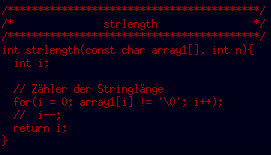
\includegraphics[width=0.9\linewidth]{images/strlength.png}
  \caption{strlength}
  \label{fig:digraph}
\end{figure}
Die Funktion 'strlength' wurde mit einer einfachen For-schleife gelöst, welche über eine variable iteriert wurde.

\begin{figure}[H]
  \centering
  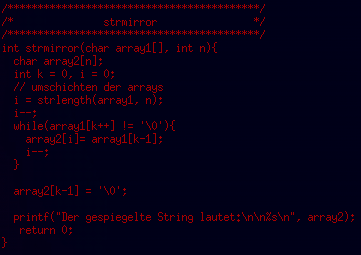
\includegraphics[width=0.9\linewidth]{images/strmirror.png}
  \caption{strmirror}
  \label{fig:digraph}
\end{figure}
Die Funktion 'strmirror' ruft zunächst strlength auf. Der Rückgabewert gibt an wie groß das Array ist. Dann wird mit einer while-Schleife nach oben gezählt bist das Nullbyte erreicht wird.

\begin{figure}[H]
  \centering
  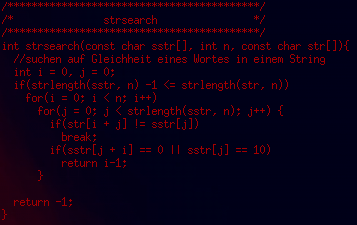
\includegraphics[width=0.9\linewidth]{images/strsearch.png}
  \caption{strsearch}
  \label{fig:digraph}
\end{figure}
Die Funktion 'strsearch' bedient sich gleich des öfteren strlength. Dies ist nötig um um Fehler vorzubeugen. Mit 'if' wird ausgeschlossen das der gesuchte String nicht größer ist als der ursprünglich String. Desweiteren wird mit dem beiden for schleifen solange nach oben gezählt bis jeder einzelne Buchstabe der beiden Strings miteinander verglichen wird. Die letzten beiden 'if'-Verzweigungen sind da um Fehler zu überprüfen bzw. die Zweite um nach einem Space zusuchen.

\begin{figure}[H]
  \centering
  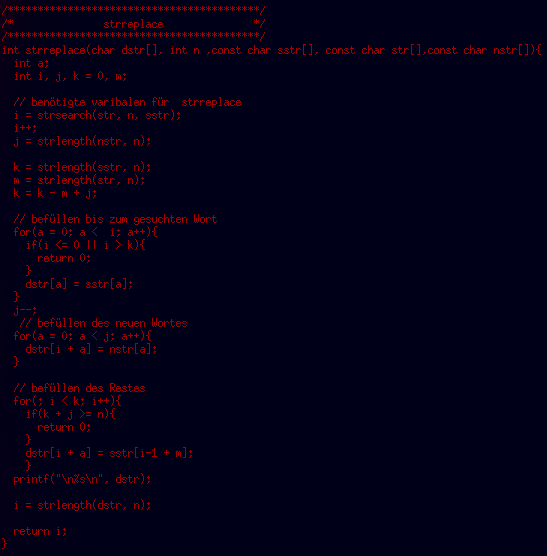
\includegraphics[width=0.9\linewidth]{images/strreplace.png}
  \caption{strreplace}
  \label{fig:digraph}
\end{figure}
Die Funktion 'strreplace' bedient sich gleich am Anfang mit 'strsearch' und öfters mit 'strlength'. Dies wird benötigt da die Rückgabewerte gebraucht werden um den neuen Array zu befüllen. Die erste 'for-Schleife' füllt das neue Array bis zum gesuchten Wort auf. Die zweite 'for-Schleife' befüllt das Array mit jenem neuen Wort das eingesetzt werden will. Die dritte 'for-Schleife' befüllt das Array mit den restlichen fehlenden Zeichen.

\begin{figure}[H]
  \centering
  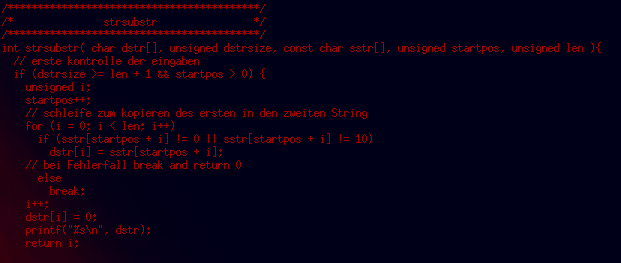
\includegraphics[width=0.9\linewidth]{images/strsubstr.png}
  \caption{strsubstr}
  \label{fig:digraph}
\end{figure}
Die Funktion 'strsubstr' überprüft im Sourcestrin ob das zu kopierende Wort vorhanden ist. Wem dem so ist kopiert es dieses in ein neues Array .
\newpage

%% Testergebnisse 
\section{Testergebnisse}
Jede Funktion wurde 3 mal mit den selben Zeichen getestet. Es wurde darauf geachtet das Groß-, Kleinbuchstaben, Zahlen sowie Sonderzeichen enthalten sind.

\subsection{Tabelle: strlength}
\begin{table}[H]
  \centering
  \begin{tabular}{|c|c|}
    \hline
    Teststring & Anzahl \\
    \hline
    Hallo erstmal & 13 \\
    \hline
    Mein Name ist Stefan & 20 \\
    \hline
    Test 123 ., & 11 \\
    \hline
  \end{tabular}
  \caption{Tabelle: strlength}
\end{table}
\subsection{Screenshot: strlength}
\begin{figure}[H]
  \centering
  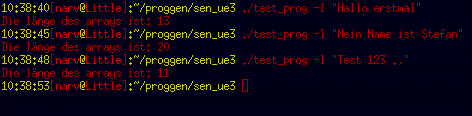
\includegraphics[width=0.9\linewidth]{images/strlength_test.png}
  \caption{strelength\_test}
  \label{fig:digraph}
\end{figure}

\newpage
\subsection{Tabelle: strmirror}
\begin{table}[H]
  \centering
  \begin{tabular}{|c|c|}
    \hline
    Teststring & Gespiegelt \\
    \hline
    Hallo erstmal & lamtsre ollaH \\
    \hline
    Mein Name ist Stefan & nafetS tsi emaN nieM \\
    \hline
    Test 123 ., & ,. 321 tseT \\
    \hline
  \end{tabular}
  \caption{Tabelle: strmirror}
\end{table}
\subsection{Screenshot: strmirror}
\begin{figure}[H]
  \centering
  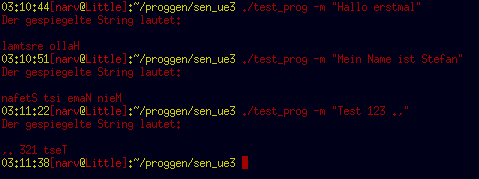
\includegraphics[width=0.9\linewidth]{images/strmirror_test.png}
  \caption{strmirror\_test}
  \label{fig:digraph}
\end{figure}

\newpage
\subsection{Tabelle: strsearch}
\begin{table}[H]
  \centering
  \begin{tabular}{|c|c|c|}
    \hline
    Teststring & zuchendes Wort & Stelle \\
    \hline
    Hallo erstmal & erstmal & 6 \\
    \hline
    Mein Name ist Stefan & Name & 5 \\
    \hline
    Test 123 ., & ., & 9 \\
    \hline
  \end{tabular}
  \caption{Tabelle: strsearch}
\end{table}
\subsection{Screenshot: strsearch}
\begin{figure}[H]
  \centering
  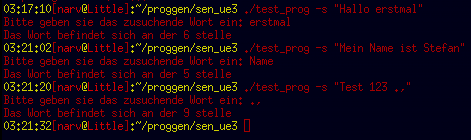
\includegraphics[width=0.9\linewidth]{images/strsearch_test.png}
  \caption{strsearch\_test}
  \label{fig:digraph}
\end{figure}

\newpage
\subsection{Tabelle: strreplace}
\begin{table}[H]
  \centering
  \begin{tabular}{|c|c|c|c|}
    \hline
    Teststring & zuchendes Wort & zuersetzendes Wort & Endstring \\
    \hline
    Hallo erstmal & erstmal & einandermal & Hallo einandermal \\
    \hline
    Mein Name ist Stefan & Name & Xylophon & Mein Xylophon ist Stefan  \\
    \hline
    Test 123 ., & ., & Test 1234. Warum nur? & Test 123 Test 1234. Warum nur?  \\
    \hline
  \end{tabular}
  \caption{Tabelle: strreplace}
\end{table}
\subsection{Screenshot: strreplace}
\begin{figure}[H]
  \centering
  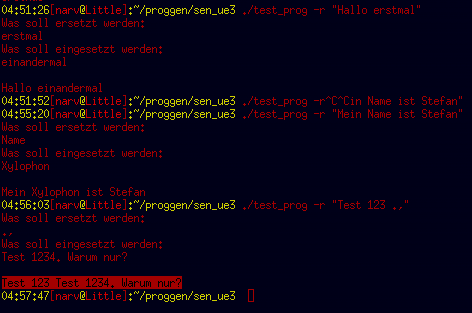
\includegraphics[width=0.9\linewidth]{images/strreplace_test.png}
  \caption{strreplace\_test}
  \label{fig:digraph}
\end{figure}

\newpage
\subsection{Tabelle: strsubstr}
\begin{table}[H]
  \centering
  \begin{tabular}{|c|c|}
    \hline
    Teststring & zukopierendes Wort \\
    \hline
    Hallo erstmal & erstmal \\
    \hline
    Mein Name ist Stefan & Name \\
    \hline
    Test 123 ., & ., \\
    \hline
  \end{tabular}
  \caption{Tabelle: strsubstr}
\end{table}
\subsection{Screenshot: strsubstr}
\begin{figure}[H]
  \centering
  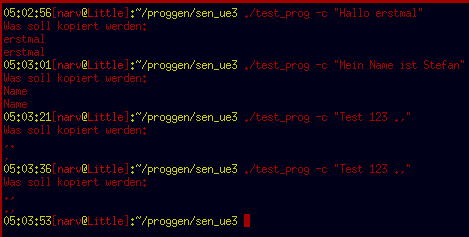
\includegraphics[width=0.9\linewidth]{images/strsubstr_test.png}
  \caption{strsubstr\_test}
  \label{fig:digraph}
\end{figure}
\end{document}
